% Created by tikzDevice version 0.12 on 2019-01-30 12:58:53
% !TEX encoding = UTF-8 Unicode
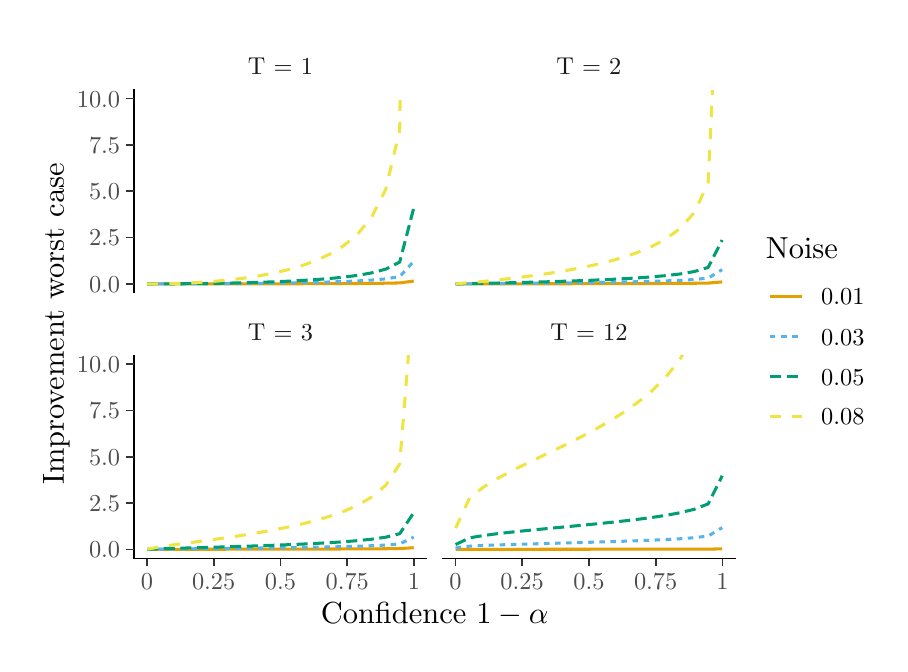
\begin{tikzpicture}[x=1pt,y=1pt]
\definecolor{fillColor}{RGB}{255,255,255}
\path[use as bounding box,fill=fillColor,fill opacity=0.00] (0,0) rectangle (307.87,222.59);
\begin{scope}
\path[clip] (  0.00,  0.00) rectangle (307.87,222.59);
\definecolor{drawColor}{RGB}{255,255,255}
\definecolor{fillColor}{RGB}{255,255,255}

\path[draw=drawColor,line width= 0.6pt,line join=round,line cap=round,fill=fillColor] (  0.00,  0.00) rectangle (307.87,222.59);
\end{scope}
\begin{scope}
\path[clip] ( 38.36,126.66) rectangle (144.32,200.29);
\definecolor{fillColor}{RGB}{255,255,255}

\path[fill=fillColor] ( 38.36,126.66) rectangle (144.32,200.29);
\definecolor{drawColor}{RGB}{230,159,0}

\path[draw=drawColor,line width= 1.1pt,line join=round] ( 43.18,130.00) --
	( 48.25,130.01) --
	( 53.32,130.01) --
	( 58.39,130.01) --
	( 63.46,130.01) --
	( 68.53,130.02) --
	( 73.60,130.02) --
	( 78.67,130.03) --
	( 83.73,130.03) --
	( 88.80,130.04) --
	( 93.87,130.05) --
	( 98.94,130.06) --
	(104.01,130.08) --
	(109.08,130.10) --
	(114.15,130.12) --
	(119.22,130.15) --
	(124.29,130.19) --
	(129.36,130.25) --
	(134.43,130.35) --
	(139.50,131.03);
\definecolor{drawColor}{RGB}{86,180,233}

\path[draw=drawColor,line width= 1.1pt,dash pattern=on 2pt off 2pt ,line join=round] ( 43.18,130.00) --
	( 48.25,130.01) --
	( 53.32,130.02) --
	( 58.39,130.03) --
	( 63.46,130.05) --
	( 68.53,130.08) --
	( 73.60,130.12) --
	( 78.67,130.16) --
	( 83.73,130.21) --
	( 88.80,130.27) --
	( 93.87,130.35) --
	( 98.94,130.44) --
	(104.01,130.55) --
	(109.08,130.69) --
	(114.15,130.86) --
	(119.22,131.08) --
	(124.29,131.38) --
	(129.36,131.82) --
	(134.43,132.63) --
	(139.50,138.17);
\definecolor{drawColor}{RGB}{0,158,115}

\path[draw=drawColor,line width= 1.1pt,dash pattern=on 4pt off 2pt ,line join=round] ( 43.18,130.00) --
	( 48.25,130.01) --
	( 53.32,130.04) --
	( 58.39,130.08) --
	( 63.46,130.13) --
	( 68.53,130.21) --
	( 73.60,130.31) --
	( 78.67,130.43) --
	( 83.73,130.58) --
	( 88.80,130.75) --
	( 93.87,130.97) --
	( 98.94,131.23) --
	(104.01,131.55) --
	(109.08,131.94) --
	(114.15,132.44) --
	(119.22,133.09) --
	(124.29,133.98) --
	(129.36,135.34) --
	(134.43,137.88) --
	(139.50,157.38);
\definecolor{drawColor}{RGB}{240,228,66}

\path[draw=drawColor,line width= 1.1pt,dash pattern=on 4pt off 4pt ,line join=round] ( 43.18,130.00) --
	( 48.25,130.04) --
	( 53.32,130.16) --
	( 58.39,130.36) --
	( 63.46,130.64) --
	( 68.53,131.03) --
	( 73.60,131.52) --
	( 78.67,132.15) --
	( 83.73,132.93) --
	( 88.80,133.89) --
	( 93.87,135.07) --
	( 98.94,136.54) --
	(104.01,138.37) --
	(109.08,140.72) --
	(114.15,143.79) --
	(119.22,147.99) --
	(124.29,154.11) --
	(129.36,164.14) --
	(134.43,185.49) --
	(134.91,222.59);
\end{scope}
\begin{scope}
\path[clip] ( 38.36, 30.72) rectangle (144.32,104.35);
\definecolor{fillColor}{RGB}{255,255,255}

\path[fill=fillColor] ( 38.36, 30.72) rectangle (144.32,104.35);
\definecolor{drawColor}{RGB}{230,159,0}

\path[draw=drawColor,line width= 1.1pt,line join=round] ( 43.18, 34.07) --
	( 48.25, 34.08) --
	( 53.32, 34.09) --
	( 58.39, 34.10) --
	( 63.46, 34.11) --
	( 68.53, 34.12) --
	( 73.60, 34.13) --
	( 78.67, 34.13) --
	( 83.73, 34.14) --
	( 88.80, 34.15) --
	( 93.87, 34.16) --
	( 98.94, 34.17) --
	(104.01, 34.19) --
	(109.08, 34.20) --
	(114.15, 34.22) --
	(119.22, 34.24) --
	(124.29, 34.26) --
	(129.36, 34.30) --
	(134.43, 34.35) --
	(139.50, 34.68);
\definecolor{drawColor}{RGB}{86,180,233}

\path[draw=drawColor,line width= 1.1pt,dash pattern=on 2pt off 2pt ,line join=round] ( 43.18, 34.08) --
	( 48.25, 34.16) --
	( 53.32, 34.22) --
	( 58.39, 34.27) --
	( 63.46, 34.33) --
	( 68.53, 34.38) --
	( 73.60, 34.44) --
	( 78.67, 34.49) --
	( 83.73, 34.56) --
	( 88.80, 34.62) --
	( 93.87, 34.69) --
	( 98.94, 34.77) --
	(104.01, 34.86) --
	(109.08, 34.95) --
	(114.15, 35.07) --
	(119.22, 35.21) --
	(124.29, 35.39) --
	(129.36, 35.63) --
	(134.43, 36.05) --
	(139.50, 38.50);
\definecolor{drawColor}{RGB}{0,158,115}

\path[draw=drawColor,line width= 1.1pt,dash pattern=on 4pt off 2pt ,line join=round] ( 43.18, 34.09) --
	( 48.25, 34.30) --
	( 53.32, 34.46) --
	( 58.39, 34.60) --
	( 63.46, 34.75) --
	( 68.53, 34.89) --
	( 73.60, 35.05) --
	( 78.67, 35.21) --
	( 83.73, 35.37) --
	( 88.80, 35.56) --
	( 93.87, 35.75) --
	( 98.94, 35.97) --
	(104.01, 36.22) --
	(109.08, 36.50) --
	(114.15, 36.82) --
	(119.22, 37.23) --
	(124.29, 37.74) --
	(129.36, 38.47) --
	(134.43, 39.72) --
	(139.50, 47.31);
\definecolor{drawColor}{RGB}{240,228,66}

\path[draw=drawColor,line width= 1.1pt,dash pattern=on 4pt off 4pt ,line join=round] ( 43.18, 34.13) --
	( 48.25, 35.09) --
	( 53.32, 35.79) --
	( 58.39, 36.46) --
	( 63.46, 37.14) --
	( 68.53, 37.83) --
	( 73.60, 38.56) --
	( 78.67, 39.34) --
	( 83.73, 40.17) --
	( 88.80, 41.08) --
	( 93.87, 42.08) --
	( 98.94, 43.21) --
	(104.01, 44.49) --
	(109.08, 45.99) --
	(114.15, 47.78) --
	(119.22, 50.01) --
	(124.29, 52.94) --
	(129.36, 57.21) --
	(134.43, 64.94) --
	(139.50,128.19);
\end{scope}
\begin{scope}
\path[clip] (149.82,126.66) rectangle (255.78,200.29);
\definecolor{fillColor}{RGB}{255,255,255}

\path[fill=fillColor] (149.82,126.66) rectangle (255.78,200.29);
\definecolor{drawColor}{RGB}{230,159,0}

\path[draw=drawColor,line width= 1.1pt,line join=round] (154.63,130.00) --
	(159.70,130.01) --
	(164.77,130.02) --
	(169.84,130.02) --
	(174.91,130.03) --
	(179.98,130.04) --
	(185.05,130.04) --
	(190.12,130.05) --
	(195.19,130.06) --
	(200.26,130.07) --
	(205.33,130.08) --
	(210.40,130.09) --
	(215.47,130.11) --
	(220.54,130.12) --
	(225.61,130.14) --
	(230.68,130.16) --
	(235.75,130.19) --
	(240.82,130.23) --
	(245.89,130.30) --
	(250.96,130.72);
\definecolor{drawColor}{RGB}{86,180,233}

\path[draw=drawColor,line width= 1.1pt,dash pattern=on 2pt off 2pt ,line join=round] (154.63,130.01) --
	(159.70,130.04) --
	(164.77,130.08) --
	(169.84,130.12) --
	(174.91,130.17) --
	(179.98,130.21) --
	(185.05,130.26) --
	(190.12,130.32) --
	(195.19,130.38) --
	(200.26,130.44) --
	(205.33,130.52) --
	(210.40,130.60) --
	(215.47,130.69) --
	(220.54,130.80) --
	(225.61,130.93) --
	(230.68,131.09) --
	(235.75,131.29) --
	(240.82,131.59) --
	(245.89,132.09) --
	(250.96,135.17);
\definecolor{drawColor}{RGB}{0,158,115}

\path[draw=drawColor,line width= 1.1pt,dash pattern=on 4pt off 2pt ,line join=round] (154.63,130.01) --
	(159.70,130.10) --
	(164.77,130.20) --
	(169.84,130.31) --
	(174.91,130.43) --
	(179.98,130.56) --
	(185.05,130.69) --
	(190.12,130.84) --
	(195.19,131.01) --
	(200.26,131.19) --
	(205.33,131.39) --
	(210.40,131.62) --
	(215.47,131.88) --
	(220.54,132.18) --
	(225.61,132.55) --
	(230.68,133.00) --
	(235.75,133.59) --
	(240.82,134.45) --
	(245.89,135.95) --
	(250.96,145.87);
\definecolor{drawColor}{RGB}{240,228,66}

\path[draw=drawColor,line width= 1.1pt,dash pattern=on 4pt off 4pt ,line join=round] (154.63,130.01) --
	(159.70,130.45) --
	(164.77,130.92) --
	(169.84,131.45) --
	(174.91,132.02) --
	(179.98,132.64) --
	(185.05,133.33) --
	(190.12,134.09) --
	(195.19,134.94) --
	(200.26,135.90) --
	(205.33,136.98) --
	(210.40,138.23) --
	(215.47,139.68) --
	(220.54,141.42) --
	(225.61,143.57) --
	(230.68,146.31) --
	(235.75,150.04) --
	(240.82,155.70) --
	(245.89,166.50) --
	(248.52,222.59);
\end{scope}
\begin{scope}
\path[clip] (149.82, 30.72) rectangle (255.78,104.35);
\definecolor{fillColor}{RGB}{255,255,255}

\path[fill=fillColor] (149.82, 30.72) rectangle (255.78,104.35);
\definecolor{drawColor}{RGB}{230,159,0}

\path[draw=drawColor,line width= 1.1pt,line join=round] (154.63, 34.08) --
	(159.70, 34.10) --
	(164.77, 34.10) --
	(169.84, 34.10) --
	(174.91, 34.11) --
	(179.98, 34.11) --
	(185.05, 34.11) --
	(190.12, 34.12) --
	(195.19, 34.12) --
	(200.26, 34.12) --
	(205.33, 34.13) --
	(210.40, 34.13) --
	(215.47, 34.13) --
	(220.54, 34.14) --
	(225.61, 34.14) --
	(230.68, 34.15) --
	(235.75, 34.15) --
	(240.82, 34.16) --
	(245.89, 34.17) --
	(250.96, 34.25);
\definecolor{drawColor}{RGB}{86,180,233}

\path[draw=drawColor,line width= 1.1pt,dash pattern=on 2pt off 2pt ,line join=round] (154.63, 34.55) --
	(159.70, 35.24) --
	(164.77, 35.49) --
	(169.84, 35.67) --
	(174.91, 35.84) --
	(179.98, 35.99) --
	(185.05, 36.13) --
	(190.12, 36.27) --
	(195.19, 36.41) --
	(200.26, 36.56) --
	(205.33, 36.70) --
	(210.40, 36.86) --
	(215.47, 37.02) --
	(220.54, 37.20) --
	(225.61, 37.40) --
	(230.68, 37.63) --
	(235.75, 37.91) --
	(240.82, 38.29) --
	(245.89, 38.89) --
	(250.96, 41.93);
\definecolor{drawColor}{RGB}{0,158,115}

\path[draw=drawColor,line width= 1.1pt,dash pattern=on 4pt off 2pt ,line join=round] (154.63, 35.82) --
	(159.70, 38.24) --
	(164.77, 39.09) --
	(169.84, 39.75) --
	(174.91, 40.32) --
	(179.98, 40.84) --
	(185.05, 41.33) --
	(190.12, 41.82) --
	(195.19, 42.30) --
	(200.26, 42.78) --
	(205.33, 43.28) --
	(210.40, 43.80) --
	(215.47, 44.35) --
	(220.54, 44.94) --
	(225.61, 45.61) --
	(230.68, 46.38) --
	(235.75, 47.31) --
	(240.82, 48.55) --
	(245.89, 50.51) --
	(250.96, 60.67);
\definecolor{drawColor}{RGB}{240,228,66}

\path[draw=drawColor,line width= 1.1pt,dash pattern=on 4pt off 4pt ,line join=round] (154.63, 41.76) --
	(159.70, 52.67) --
	(164.77, 56.64) --
	(169.84, 59.72) --
	(174.91, 62.42) --
	(179.98, 64.95) --
	(185.05, 67.39) --
	(190.12, 69.83) --
	(195.19, 72.30) --
	(200.26, 74.87) --
	(205.33, 77.57) --
	(210.40, 80.48) --
	(215.47, 83.67) --
	(220.54, 87.26) --
	(225.61, 91.41) --
	(230.68, 96.41) --
	(235.75,102.83) --
	(240.82,111.93) --
	(245.89,127.97) --
	(249.47,222.59);
\end{scope}
\begin{scope}
\path[clip] ( 38.36,104.35) rectangle (144.32,121.16);
\definecolor{drawColor}{RGB}{255,255,255}
\definecolor{fillColor}{RGB}{255,255,255}

\path[draw=drawColor,line width= 1.1pt,line join=round,line cap=round,fill=fillColor] ( 38.36,104.35) rectangle (144.32,121.16);
\definecolor{drawColor}{gray}{0.10}

\node[text=drawColor,anchor=base,inner sep=0pt, outer sep=0pt, scale=  0.88] at ( 91.34,109.73) {T = 3};
\end{scope}
\begin{scope}
\path[clip] (149.82,104.35) rectangle (255.78,121.16);
\definecolor{drawColor}{RGB}{255,255,255}
\definecolor{fillColor}{RGB}{255,255,255}

\path[draw=drawColor,line width= 1.1pt,line join=round,line cap=round,fill=fillColor] (149.82,104.35) rectangle (255.78,121.16);
\definecolor{drawColor}{gray}{0.10}

\node[text=drawColor,anchor=base,inner sep=0pt, outer sep=0pt, scale=  0.88] at (202.80,109.73) {T = 12};
\end{scope}
\begin{scope}
\path[clip] ( 38.36,200.29) rectangle (144.32,217.09);
\definecolor{drawColor}{RGB}{255,255,255}
\definecolor{fillColor}{RGB}{255,255,255}

\path[draw=drawColor,line width= 1.1pt,line join=round,line cap=round,fill=fillColor] ( 38.36,200.29) rectangle (144.32,217.09);
\definecolor{drawColor}{gray}{0.10}

\node[text=drawColor,anchor=base,inner sep=0pt, outer sep=0pt, scale=  0.88] at ( 91.34,205.66) {T = 1};
\end{scope}
\begin{scope}
\path[clip] (149.82,200.29) rectangle (255.78,217.09);
\definecolor{drawColor}{RGB}{255,255,255}
\definecolor{fillColor}{RGB}{255,255,255}

\path[draw=drawColor,line width= 1.1pt,line join=round,line cap=round,fill=fillColor] (149.82,200.29) rectangle (255.78,217.09);
\definecolor{drawColor}{gray}{0.10}

\node[text=drawColor,anchor=base,inner sep=0pt, outer sep=0pt, scale=  0.88] at (202.80,205.66) {T = 2};
\end{scope}
\begin{scope}
\path[clip] (  0.00,  0.00) rectangle (307.87,222.59);
\definecolor{drawColor}{RGB}{0,0,0}

\path[draw=drawColor,line width= 0.6pt,line join=round] ( 38.36, 30.72) --
	(144.32, 30.72);
\end{scope}
\begin{scope}
\path[clip] (  0.00,  0.00) rectangle (307.87,222.59);
\definecolor{drawColor}{gray}{0.20}

\path[draw=drawColor,line width= 0.6pt,line join=round] ( 43.08, 27.97) --
	( 43.08, 30.72);

\path[draw=drawColor,line width= 0.6pt,line join=round] ( 67.21, 27.97) --
	( 67.21, 30.72);

\path[draw=drawColor,line width= 0.6pt,line join=round] ( 91.34, 27.97) --
	( 91.34, 30.72);

\path[draw=drawColor,line width= 0.6pt,line join=round] (115.47, 27.97) --
	(115.47, 30.72);

\path[draw=drawColor,line width= 0.6pt,line join=round] (139.60, 27.97) --
	(139.60, 30.72);
\end{scope}
\begin{scope}
\path[clip] (  0.00,  0.00) rectangle (307.87,222.59);
\definecolor{drawColor}{gray}{0.30}

\node[text=drawColor,anchor=base,inner sep=0pt, outer sep=0pt, scale=  0.88] at ( 43.08, 19.71) {0};

\node[text=drawColor,anchor=base,inner sep=0pt, outer sep=0pt, scale=  0.88] at ( 67.21, 19.71) {0.25};

\node[text=drawColor,anchor=base,inner sep=0pt, outer sep=0pt, scale=  0.88] at ( 91.34, 19.71) {0.5};

\node[text=drawColor,anchor=base,inner sep=0pt, outer sep=0pt, scale=  0.88] at (115.47, 19.71) {0.75};

\node[text=drawColor,anchor=base,inner sep=0pt, outer sep=0pt, scale=  0.88] at (139.60, 19.71) {1};
\end{scope}
\begin{scope}
\path[clip] (  0.00,  0.00) rectangle (307.87,222.59);
\definecolor{drawColor}{RGB}{0,0,0}

\path[draw=drawColor,line width= 0.6pt,line join=round] (149.82, 30.72) --
	(255.78, 30.72);
\end{scope}
\begin{scope}
\path[clip] (  0.00,  0.00) rectangle (307.87,222.59);
\definecolor{drawColor}{gray}{0.20}

\path[draw=drawColor,line width= 0.6pt,line join=round] (154.54, 27.97) --
	(154.54, 30.72);

\path[draw=drawColor,line width= 0.6pt,line join=round] (178.67, 27.97) --
	(178.67, 30.72);

\path[draw=drawColor,line width= 0.6pt,line join=round] (202.80, 27.97) --
	(202.80, 30.72);

\path[draw=drawColor,line width= 0.6pt,line join=round] (226.93, 27.97) --
	(226.93, 30.72);

\path[draw=drawColor,line width= 0.6pt,line join=round] (251.06, 27.97) --
	(251.06, 30.72);
\end{scope}
\begin{scope}
\path[clip] (  0.00,  0.00) rectangle (307.87,222.59);
\definecolor{drawColor}{gray}{0.30}

\node[text=drawColor,anchor=base,inner sep=0pt, outer sep=0pt, scale=  0.88] at (154.54, 19.71) {0};

\node[text=drawColor,anchor=base,inner sep=0pt, outer sep=0pt, scale=  0.88] at (178.67, 19.71) {0.25};

\node[text=drawColor,anchor=base,inner sep=0pt, outer sep=0pt, scale=  0.88] at (202.80, 19.71) {0.5};

\node[text=drawColor,anchor=base,inner sep=0pt, outer sep=0pt, scale=  0.88] at (226.93, 19.71) {0.75};

\node[text=drawColor,anchor=base,inner sep=0pt, outer sep=0pt, scale=  0.88] at (251.06, 19.71) {1};
\end{scope}
\begin{scope}
\path[clip] (  0.00,  0.00) rectangle (307.87,222.59);
\definecolor{drawColor}{RGB}{0,0,0}

\path[draw=drawColor,line width= 0.6pt,line join=round] ( 38.36,126.66) --
	( 38.36,200.29);
\end{scope}
\begin{scope}
\path[clip] (  0.00,  0.00) rectangle (307.87,222.59);
\definecolor{drawColor}{gray}{0.30}

\node[text=drawColor,anchor=base east,inner sep=0pt, outer sep=0pt, scale=  0.88] at ( 33.41,126.97) {0.0};

\node[text=drawColor,anchor=base east,inner sep=0pt, outer sep=0pt, scale=  0.88] at ( 33.41,143.71) {2.5};

\node[text=drawColor,anchor=base east,inner sep=0pt, outer sep=0pt, scale=  0.88] at ( 33.41,160.44) {5.0};

\node[text=drawColor,anchor=base east,inner sep=0pt, outer sep=0pt, scale=  0.88] at ( 33.41,177.18) {7.5};

\node[text=drawColor,anchor=base east,inner sep=0pt, outer sep=0pt, scale=  0.88] at ( 33.41,193.91) {10.0};
\end{scope}
\begin{scope}
\path[clip] (  0.00,  0.00) rectangle (307.87,222.59);
\definecolor{drawColor}{gray}{0.20}

\path[draw=drawColor,line width= 0.6pt,line join=round] ( 35.61,130.00) --
	( 38.36,130.00);

\path[draw=drawColor,line width= 0.6pt,line join=round] ( 35.61,146.74) --
	( 38.36,146.74);

\path[draw=drawColor,line width= 0.6pt,line join=round] ( 35.61,163.47) --
	( 38.36,163.47);

\path[draw=drawColor,line width= 0.6pt,line join=round] ( 35.61,180.21) --
	( 38.36,180.21);

\path[draw=drawColor,line width= 0.6pt,line join=round] ( 35.61,196.94) --
	( 38.36,196.94);
\end{scope}
\begin{scope}
\path[clip] (  0.00,  0.00) rectangle (307.87,222.59);
\definecolor{drawColor}{RGB}{0,0,0}

\path[draw=drawColor,line width= 0.6pt,line join=round] ( 38.36, 30.72) --
	( 38.36,104.35);
\end{scope}
\begin{scope}
\path[clip] (  0.00,  0.00) rectangle (307.87,222.59);
\definecolor{drawColor}{gray}{0.30}

\node[text=drawColor,anchor=base east,inner sep=0pt, outer sep=0pt, scale=  0.88] at ( 33.41, 31.04) {0.0};

\node[text=drawColor,anchor=base east,inner sep=0pt, outer sep=0pt, scale=  0.88] at ( 33.41, 47.77) {2.5};

\node[text=drawColor,anchor=base east,inner sep=0pt, outer sep=0pt, scale=  0.88] at ( 33.41, 64.51) {5.0};

\node[text=drawColor,anchor=base east,inner sep=0pt, outer sep=0pt, scale=  0.88] at ( 33.41, 81.24) {7.5};

\node[text=drawColor,anchor=base east,inner sep=0pt, outer sep=0pt, scale=  0.88] at ( 33.41, 97.98) {10.0};
\end{scope}
\begin{scope}
\path[clip] (  0.00,  0.00) rectangle (307.87,222.59);
\definecolor{drawColor}{gray}{0.20}

\path[draw=drawColor,line width= 0.6pt,line join=round] ( 35.61, 34.07) --
	( 38.36, 34.07);

\path[draw=drawColor,line width= 0.6pt,line join=round] ( 35.61, 50.81) --
	( 38.36, 50.81);

\path[draw=drawColor,line width= 0.6pt,line join=round] ( 35.61, 67.54) --
	( 38.36, 67.54);

\path[draw=drawColor,line width= 0.6pt,line join=round] ( 35.61, 84.27) --
	( 38.36, 84.27);

\path[draw=drawColor,line width= 0.6pt,line join=round] ( 35.61,101.01) --
	( 38.36,101.01);
\end{scope}
\begin{scope}
\path[clip] (  0.00,  0.00) rectangle (307.87,222.59);
\definecolor{drawColor}{RGB}{0,0,0}

\node[text=drawColor,anchor=base,inner sep=0pt, outer sep=0pt, scale=  1.10] at (147.07,  7.44) {Confidence $1 - \alpha$};
\end{scope}
\begin{scope}
\path[clip] (  0.00,  0.00) rectangle (307.87,222.59);
\definecolor{drawColor}{RGB}{0,0,0}

\node[text=drawColor,rotate= 90.00,anchor=base,inner sep=0pt, outer sep=0pt, scale=  1.10] at ( 13.08,115.51) {Improvement worst case};
\end{scope}
\begin{scope}
\path[clip] (  0.00,  0.00) rectangle (307.87,222.59);
\definecolor{fillColor}{RGB}{255,255,255}

\path[fill=fillColor] (266.78, 86.20) rectangle (302.37,144.81);
\end{scope}
\begin{scope}
\path[clip] (  0.00,  0.00) rectangle (307.87,222.59);
\definecolor{drawColor}{RGB}{0,0,0}

\node[text=drawColor,anchor=base west,inner sep=0pt, outer sep=0pt, scale=  1.10] at (266.78,139.11) {Noise};
\end{scope}
\begin{scope}
\path[clip] (  0.00,  0.00) rectangle (307.87,222.59);
\definecolor{drawColor}{RGB}{230,159,0}

\path[draw=drawColor,line width= 1.1pt,line join=round] (268.22,125.41) -- (279.78,125.41);
\end{scope}
\begin{scope}
\path[clip] (  0.00,  0.00) rectangle (307.87,222.59);
\definecolor{drawColor}{RGB}{86,180,233}

\path[draw=drawColor,line width= 1.1pt,dash pattern=on 2pt off 2pt ,line join=round] (268.22,110.95) -- (279.78,110.95);
\end{scope}
\begin{scope}
\path[clip] (  0.00,  0.00) rectangle (307.87,222.59);
\definecolor{drawColor}{RGB}{0,158,115}

\path[draw=drawColor,line width= 1.1pt,dash pattern=on 4pt off 2pt ,line join=round] (268.22, 96.50) -- (279.78, 96.50);
\end{scope}
\begin{scope}
\path[clip] (  0.00,  0.00) rectangle (307.87,222.59);
\definecolor{drawColor}{RGB}{240,228,66}

\path[draw=drawColor,line width= 1.1pt,dash pattern=on 4pt off 4pt ,line join=round] (268.22, 82.05) -- (279.78, 82.05);
\end{scope}
\begin{scope}
\path[clip] (  0.00,  0.00) rectangle (307.87,222.59);
\definecolor{drawColor}{RGB}{0,0,0}

\node[text=drawColor,anchor=base west,inner sep=0pt, outer sep=0pt, scale=  0.88] at (286.73,122.38) {0.01};
\end{scope}
\begin{scope}
\path[clip] (  0.00,  0.00) rectangle (307.87,222.59);
\definecolor{drawColor}{RGB}{0,0,0}

\node[text=drawColor,anchor=base west,inner sep=0pt, outer sep=0pt, scale=  0.88] at (286.73,107.92) {0.03};
\end{scope}
\begin{scope}
\path[clip] (  0.00,  0.00) rectangle (307.87,222.59);
\definecolor{drawColor}{RGB}{0,0,0}

\node[text=drawColor,anchor=base west,inner sep=0pt, outer sep=0pt, scale=  0.88] at (286.73, 93.47) {0.05};
\end{scope}
\begin{scope}
\path[clip] (  0.00,  0.00) rectangle (307.87,222.59);
\definecolor{drawColor}{RGB}{0,0,0}

\node[text=drawColor,anchor=base west,inner sep=0pt, outer sep=0pt, scale=  0.88] at (286.73, 79.02) {0.08};
\end{scope}
\end{tikzpicture}
